\tikzset{every picture/.style={line width=0.75pt}}      

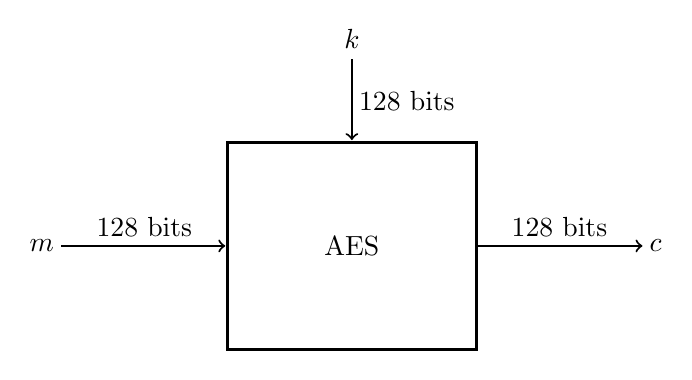
\begin{tikzpicture}[x=0.75pt,y=0.75pt,yscale=-1,xscale=1]

\draw  [line width=1.2]  (100,60) -- (220,60) -- (220,160) -- (100,160) -- cycle ;

\draw  [->]  (20,110) -- (99,110) ;
\draw  [->]  (220,110) -- (300,110) ;
\draw  [->]  (160,20) -- (160,59) ;

\draw (160,110) node   [align=left] {AES};
\draw (60,107) node [anchor=south] [inner sep=0.75pt]   [align=left] {$ 128$ bits};
\draw (260,107) node [anchor=south] [inner sep=0.75pt]   [align=left] {$ 128$ bits};
\draw (162,40) node [anchor=west] [inner sep=0.75pt]   [align=left] {$ 128$ bits};
\draw (18,110) node [anchor=east] [inner sep=0.75pt]    {$m$};
\draw (302,110) node [anchor=west] [inner sep=0.75pt]    {$c$};
\draw (160,16.6) node [anchor=south] [inner sep=0.75pt]    {$k$};


\end{tikzpicture}